\documentclass[12pt,draftcls,onecolumn]{IEEEtran}

\usepackage{amsmath}
\usepackage{amssymb}
\usepackage{graphicx}
%\usepackage[margin=1in]{geometry}
\usepackage{ulem}
\usepackage{subcaption}

% Daniel definitions
\def \rmT {\mathrm{T}}
\def \trans {^\rmT} 
\def \prior {^-}
\def \post {^+}
\def \k {(k)}
\def \kone {(k+1)}
\def \x {\mathrm{\mathbf{x}}}
\def \v {\mathrm{\mathbf{v}}}
\def \y {\mathrm{\mathbf{y}}}
\def \ytilde {\tilde\y}
\def \w {\mathrm{\mathbf{w}}}
\def \u {\mathrm{\mathbf{u}}}
\def \xhat {\hat{\x}}
\def \xtilde {\tilde{\x}}
\def \xkhat {\xhat\k }
\def \ykhat {\hat\y\k }
\def \xkonehat {\xhat\kone }
\def \xk {\x\k }
\def \xprior {\hat\x\prior }
\def \xpost {\hat\x\post }
\def \yktilde {\ytilde\k }
\def \uk {\u\k }
\def \wk {\w\k }
\def \vk {\v\k }
\def \xkone {\x\kone }
\def \Phik {\Phi\k }
\def \Qk {\mathrm{Q}\k }
\def \Kk {\mathrm{K}\k }
\def \Hk {\mathrm{H}\k }
\def \Pk {\mathrm{P}_{xx,k}}
\def \Pxx {\mathrm{P}_{xx}}
\def \Pyy {\mathrm{P}_{yy}}
\def \Pxy {\mathrm{P}_{xy}}
\def \Gammak {\Gamma\k }
\def \Rk {\mathrm{R}\k }
\def \Upsilonk {\Upsilon\k }
\def \terma {\big(\mathrm{I} -\Kk\Hk\big)}

% Tim macros
\newcommand{\ddarg}[2]{\ensuremath{\frac{d#1}{d#2}}}
\newcommand{\pparg}[2]{\ensuremath{\frac{\partial #1}{\partial #2}}}

\newcommand{\pip}{\ensuremath{\Bigg |}}
\renewcommand{\vec}[1]{\ensuremath{\mathrm{\mathbf{#1}}}}
\newcommand{\vecin}[2]{\ensuremath{\mathrm{\mathbf{#1}}}(#2)}
\newcommand{\ten}[1]{\ensuremath{\mathrm{#1}}}
\newcommand{\symvec}[1]{\ensuremath{\mathrm{\boldsymbol{#1}}}}

\newcommand{\f}{{\symvec{\phi}}}
\newcommand{\F}{{\ten{\Phi}}}
\newcommand{\G}{{\ten{G}}}
\renewcommand{\H}{{\ten{\Upsilon}}}
\newcommand{\h}{{\symvec{\upsilon}}}
\newcommand{\B}{{\ten{\Gamma}}}
\renewcommand{\P}{{\ten{P_{xx}}}}

\author{Kiran Vishnu, Daniel Whitten, Tim Woodbury}
\title{ECEN 662 Group Report: Overview of the Kalman Filter and Some Common Extensions}

\begin{document}

\maketitle

\begin{abstract}
The Kalman filter has a storied history in the estimation of correlated-in-time processes.
In Kalman's original work, the filter estimate was shown to be optimal in a minimum mean square error sense for Gaussian systems. It was further shown that the optimal estimate for a sequence of measurements could be realized by operating the filter sequentially, treating only one measurement at a time.
In the present work, the linear Kalman filter is reviewed.
A simple numerical example is presented to demonstrate the implementation of the filter.
Subsequently, a discussion of two extensions of the Kalman filter to nonlinear systems is given.
These methods are the Extended Kalman Filter, in which the nonlinear system is replaced by a two-term Taylor series expansion, and the Unscented Kalman Filter, in which the estimate distribution is approximated by deterministically defined particles.
The equations governing the nonlinear approximations are given, and the two filters are discussed at a high level.
\end{abstract}

\section{Introduction}

The Kalman filter's origins trace back to 1960 and Kalman's distinguished work \cite{kalman1960}.
The contribution of the paper is difficult to overstate; few methods in engineering have received so much attention, or been applied to so many diverse problems.
Kalman showed that the optimal filter for a linear system with Gaussian forcing could be expressed as a sequential linear function of a prior and measurements.
As a consequence, the optimal estimate at time $k$ given all the measurements at $t = 0, 1, \dots, k-1$ is equivalent to the optimal estimate at time $k$ given the measurement at $k-1$ and the optimal estimate at time $k-1$.
This has profound implications in terms of data reduction and, in an era of relatively limited computer memory, enabled many online estimation problems to be solved.

Many practical systems of interest are nonlinear, state-dependent processes.
It has long been desired to extend the utility and simplicity of the Kalman filter to such systems.
Unfortunately, the optimal estimate for nonlinear systems in general is intractable\cite{kay1993}.
Two popular approaches to approximate the Kalman filter for nonlinear systems are the Extended Kalman Filter (EKF) and the Unscented Kalman Filter (UKF).
The EKF is a classic approach in which the Kalman Filter is linearized about a prior state at each cycle of prediction and update.
The EKF has been widely used and has many attactive qualities, but it is known to perform poorly for certain types of problems\cite{wan2000}.
The UKF replaces the prior state and covariance by a particle approximation.
However, unlike in other particle filters, the UKF points are deterministic functions of the prior, and the number of points is of the same order as the size of the state vector.
The result is a nonlinear estimate that better approximates the true system statistics than the EKF, at a typically higher computational cost.

In this document, a short derivation of the Kalman Filter from a dynamic systems perspective is given.
A brief simulation example is shown, demonstrating the simplicity of the filter.
Subsequently, a discussion of the EKF and UKF is presented.

\section{The Linear Discrete Kalman Filter}

The original Kalman filter considers a linear discrete dynamic model and a linear discrete measurement model.

\subsection{System Models}
The discrete dynamic model relates the state at some time $ k $ to the state at the current time $ k+1 $.
This is also known as the process model.

\begin{equation}
\xkone=\Phik\xk+\Gammak\uk + \Upsilonk\wk
\end{equation}
$\xk$ is some state of interest at time k.
$\uk$ is a deterministic input vector.
$\wk $ is zero-mean Guassian white-noise process with 
\begin{equation}
E[\wk\wk]=\Qk 
\end{equation}
\begin{equation}
E[\wk\w(j)]=\mathbf{0}  \quad j \neq k
\end{equation}

It is useful to find the first and second moments of these models.
\begin{equation}
E[\xkone]=\xprior\kone  =\Phik\xkhat+\Gammak\uk
\end{equation}
\begin{equation}
Cov[\xkone,\xkone]=\Pxx\prior\kone =\Phik\Pxx\k\Phik\trans +\Upsilonk\Qk\Upsilonk\trans 
\end{equation}

$ \xprior\kone $ and $ \Pxx\prior\kone $ can be used to predict the state at time $ k+1 $ given the state at $ k$.

A measurement vector $ \yktilde $ is available.
$ \yktilde $ relates to the state according to 

\begin{equation}
\yktilde=\Hk\xk+\vk
\end{equation}
\begin{equation}
E[\vk\vk]=\Rk 
\end{equation}

A measurement estimate $ \ykhat $ is found by taking the expectation of this model

\begin{equation}
E[\yktilde]=\hat\y\k=\Hk\xprior\k
\end{equation}

It is also useful to define and determine the second moments of this model
\begin{equation}
Cov[\yktilde,\yktilde]=\Pyy\k=\Hk\Pxx\prior\k\Hk\trans+\Rk
\end{equation}
\begin{equation}
Cov[\xk,\yktilde]=\Pxy\k=\Pxx\prior\k\Hk
\end{equation}

\subsection{Minimum Mean Square}
When a measurement $ \yktilde $ becomes available, the process model can be used to predict, or propagate, the state estimate from the previous time to the current time.
This is known as the prior estimate $ \xprior\k $.
It is desirable to update the state estimate $ \xprior\k $ using the information about the state provided by the measurement. 
This updated measurement, $ \xpost\k $, is known as the posterior estimate.

The update equations will first be developed by assuming an estimator in the form of a sequential linear estimator with a gain $ \Kk $ and then finding $ \Kk $ to minimize the mean square error (MSE).
It will then be shown that if the initial state is Guassian then this estimator is also the minimum mean square error (MMSE) estimator.

The updated state $ \xpost\k $ estimator is assumed to be in the form of a linear sequential estimator. 
\begin{equation}
\xpost\k = \xprior\k + \Kk\big(\yktilde-\ykhat\big)
\end{equation}

It is necessary to find $ \Kk $ so that $ \xhat\k\post $ minimizes some performance criteria. 
The mean square error is a natural choice. 
\begin{equation}
 MSE=\Pxx\post\k=E\big[\big(\xk-\xpost\k\big)\big(\xk-\xpost\k\big)\trans\big]
\end{equation}

By using the previously defined value of  $ \xprior\k $, the error $ \big(\xk-\xpost\k\big) $ can be written as
\begin{equation}
\xk-\xpost\k = \terma \big(\xk-\xkhat\big) + \Kk\vk
\end{equation}

After expanding out the terms of the square error and finding its expected value
\begin{equation}
\Pxx\post\k=\terma \Pxx\prior\k \terma \trans+\Kk\Rk\Kk
\end{equation}

To minimize MSE, it is equivalent to minimize the trace of $\Pxx\post$.
\begin{equation}
J=trace(\Pxx\post)
\end{equation}

Finding the partial derivative of $ J $ with respect to $ \Kk $
\begin{equation}
\frac{\partial J}{\partial \Kk} = 0 = -2\terma \Pxx\prior\k\Hk\trans+2\Kk\Rk
\end{equation}

Solving for $\Kk$
\begin{equation}
\Kk =\Pxx\prior\k\Hk\trans\big(\Hk\Pxx\prior\k\Hk\trans+\Rk\big)^{-1} 
\end{equation}

This choice of $\Kk $ minimizes the MSE for a linear estimator.
That is, the Kalman filter provides the optimal \textit{linear} MMSE estimate.

If the initial state is sampled from a normal distribution, the state remains linear because a Gaussian random variable that undergoes linear transformations remains linear. 
In this case, $\xk$ and $\yktilde$ are jointly Guassian

The MMSE estimator is known to be 
\begin{equation}
\xhat_{MMSE}\k=E[\xk|\yktilde]
\end{equation}

It is well known that for jointly Gaussian $ \xk $ and $ \yktilde $ 
\begin{equation}
E[\xk|\yktilde]=E[\xk]+\Pxy\k\Pyy^{-1}\k\big(\yktilde-E[\yktilde]\big)
\end{equation}

Having previously defined each term of this equation in terms of the process and measurement model, it can be re-written as 
\begin{equation}
E[\xk|\yktilde]=\xprior\k+\bigg(\Pxx\prior\k\Hk\trans\big(\Hk\Pxx\prior\k\Hk\trans+\Rk\big)^{-1}\bigg) \big(\yktilde-\Hk\xprior\k\big)
\end{equation}
\begin{equation}
E[\xk|\yktilde]=\xprior\k+\Kk \big(\yktilde-\Hk\xprior\k\big)
\end{equation}

Thus, for a Gaussian state prior, the Kalman filter is the MMSE estimator. 

\subsection{Algorithm Summary}

The linear discrete Kalman filter can be described and implemented in three distinct stages.

Initialize:
\begin{equation}
\xhat(t_0)=\xhat_0 
\end{equation}
\begin{equation}
\Pxx(t_0)=Cov[\xhat_0,\xhat_0]
\end{equation}

Predict:
\begin{equation}
\xprior\kone  =\Phik\xkhat+\Gammak\uk
\end{equation}
\begin{equation}
\Pxx\prior\kone =\Phik\Pxx\k\Phik\trans +\Upsilonk\Qk\Upsilonk\trans
\end{equation}

Update:
\begin{equation}
\Kk =\Pxx\prior\k\Hk\trans\big(\Hk\Pxx\prior\k\Hk\trans+\Rk\big)^{-1}
\end{equation}
\begin{equation}
\xpost\k = \xprior\k + \Kk\big(\yktilde-\ykhat\big) 
\end{equation}
\begin{equation}
\Pxx\post\k=\big(\mathrm{I}-\Kk\Hk\big)\Pxx\prior\k
\end{equation}

Using the models:
\begin{equation}
\xkone=\Phik\xk+\Gammak\uk + \Upsilonk\wk \qquad \wk\sim N\big(\mathbf{0},\Qk\big)
\end{equation}
\begin{equation}
\yktilde=\Hk\xk+\vk \qquad \vk\sim N\big(\mathbf{0},\Rk\big)
\end{equation}

This section has introduced the linear Kalman Filter and justified its optimality in a MMSE sense.
The next section presents a numerical implementation of the Kalman Filter.

\section{Kalman Filter simulation}

Consider a simple linear system with known analytical solution: a projectile launched with an initial velocity, falling under the influence of a constant gravity, with no air resistance.
The gravitational acceleration is treated as a deterministic input.
The $y$ axis is taken as normal to the ground, leading to the following true dynamics for the position states $x,y$ and velocities $v_x,v_y$:
\begin{align}
\dot{x} = v_x \\
\dot{v_x} = 0 \\
\dot{y} = v_y \\
\dot{v_y} = -g \\
\xk \equiv \begin{bmatrix} x\k & v_x\k & y\k & v_y\k \end{bmatrix}^T
\end{align}

The initial states are chosen such that $v_x = v_y \approx 70.7$ m/s, and the gravitational acceleration is taken as a constant $9.81$ m/s$^2$.
The system is discretized with a simple Euler integration model at $\Delta T = 0.01$ seconds, leading to the following discrete-time process model:

\begin{equation}
\xkone = \begin{bmatrix}
1 & \Delta T & 0 & 0\\
0 & 1 & 0 & 0\\
0 & 0 & 1 & \Delta T\\
0 & 0 & 0 & 1
\end{bmatrix}\xk + 
\begin{bmatrix}
0 \\ 0 \\ 0 \\ -\Delta T
\end{bmatrix} g
\end{equation}

Note that no explicit process noise is included in the dynamics.
However, the simulated states are evaluated using the analytical solution, which leads to a discretization error due to the use of Euler integration.
This discretization error is modeled as a zero-mean process with the following covariance:

\begin{equation}
\Qk = \mathrm{diag}\begin{bmatrix} \Delta T^{0.25} & \Delta T & \Delta T & \Delta T \end{bmatrix}
\end{equation}

This covariance was tuned experimentally to produce more consistent filter outputs.
The measurement matrix is taken simply to be identity, with linear measurements of the full state.
The measurement covariance matrix is diagonal with each measurement having variance 10.
Python simulation results are now presented.

\begin{figure}[tb!]
\centering
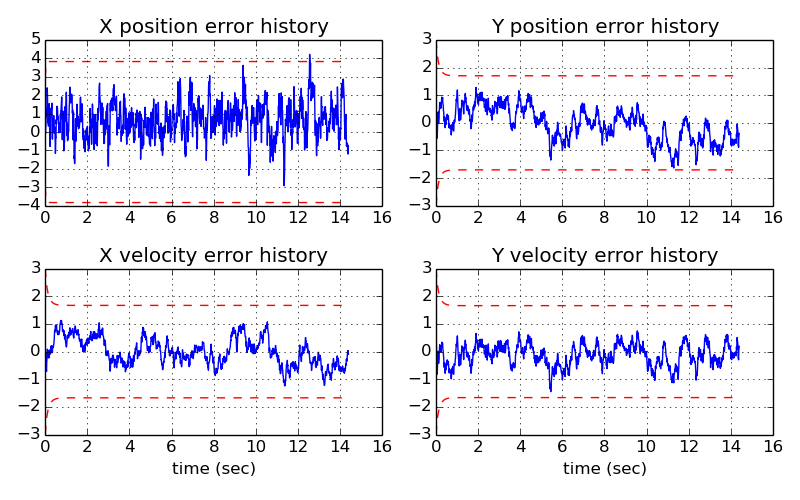
\includegraphics[width=\textwidth]{kf_errors}
\caption{Kalman filter errors relative to truth. $3\times$ the square root of covariance diagonals plotted in red for reference.}
\label{fig:kf_errors}
\end{figure}

\begin{figure}[tb!]
\centering
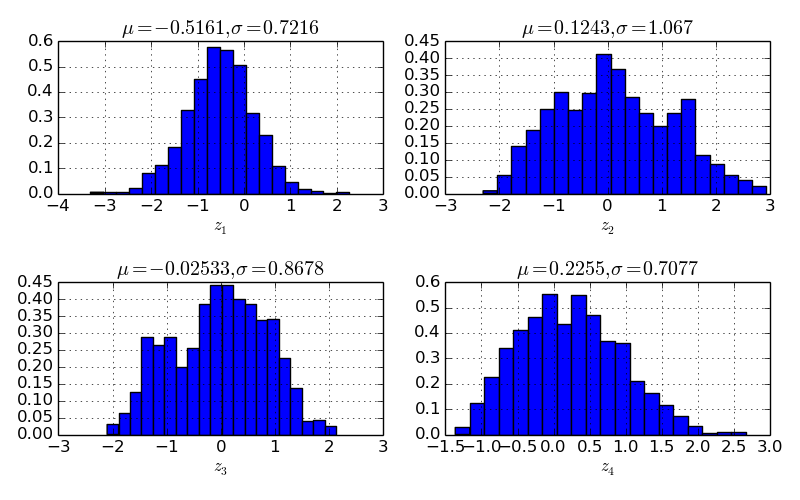
\includegraphics[width=\textwidth]{kf_consistency}
\caption{Histograms of normalized filter states.}
\label{fig:kf_consistency}
\end{figure}

For brevity, we show only the filter tracking errors (Fig. \ref{fig:kf_errors}) and consistency histograms (Fig. \ref{fig:kf_consistency}).
The tracking errors are simply the difference between the filter states and true states at each moment in time.
Three times the square root of the covariance diagonal elements is plotted as a metric of filter accuracy and consistency.
The filter appears to be somewhat conservative, since the errors are typically less than the $3\sigma$ approximations.
However, the $x$ position history shows a bias.
No doubt this bias is largely attributable to the use of first-order discretized integration.

For Fig. \ref{fig:kf_consistency}, the filter errors are regularized to states $\vec{z}$ having expected mean and covariance $0,1$: $\vec{z} \equiv \ten{P}^{1/2}(\vec{x}-\vec{\hat{x}})$.
If the filter is consistent, the regularized states $\vec{z}$ should be zero-mean and have unit variance.
In Fig. \ref{fig:kf_consistency}, histograms of the regularized states are plotted.
Note that states $z_1,z_2,z_3,z_4$ correspond approximately to x position, x velocity, y position, and y velocity.
It is clear that the states are approximately Gaussian but with some error.
In particular, the $z_1$ and $z_4$ states exhibit a noticeable bias and the filter is conservative, because the actual variance is less than 1.
The $z_2$ and $z_4$ states are more consistent.

Overall, the filter implementation is imperfect, but adequate for the purposes of demonstrating the basics of the Kalman Filter.
The following section explores advanced topics in nonlinear sequential estimation.

\section{Advanced topics}

In many processes of interest in practical problems, the strict assumptions of a linear system with Gaussian process and measurement noise are not satisfied.
For instance, consider the radar tracking problem: radar will usually measure the range and bearing and elevation angles to a target.
The measurement noise is not likely to be perfectly Gaussian.
One can either write the target dynamic equations in terms of range and angles (in which case the dynamics are nonlinear); or, one may compute 3-dimensional coordinates $x,y,z$ from the raw measurements, in which case the measurement noise undergoes a nonlinear transformation.
There is no perfect general transformation that allows the strict assumptions of linear dynamics and linear measurements to be guaranteed. This motivates the need for nonlinear estimators.

Perhaps the most intuitive approach to the nonlinear estimation problem is to linearize the nonlinear system about the prior state, and use the Jacobians of the system in the Kalman covariance equations.
This process is the EKF, and is widely used for nonlinear estimation in many fields including aerospace and process engineering.
The linearized approximation, however, may fail in some cases, particularly if an accurate prior for the estimate is not known.
This has motivated the developement of other techniques.
The UKF, sometimes called the Sigma Point Filter, uses a discrete approximation to the prior density.
The literature indicates that this approximation is more accurate than the linearization of the EKF \cite{wan2000}.
The remainder of this section presents an overview of the EKF and UKF.
We begin with a presentation of the EKF.

\subsection{Extended Kalman Filter}

This discussion is motivated by Ref. \cite{crassidis2011}.
Consider a generic discrete nonlinear system with discrete nonlinear measurements and discrete controls $\vecin{u}{k}$, and a Gaussian prior for the estimated state.
Let $\vecin{w}{k}$ and $\vecin{v}{k}$ indicate zero-mean process noise and measurement noise:
\begin{equation}
\vecin{x}{k+1} = \f(\vecin{x}{k},\vecin{u}{k}) + \G(k) \vecin{w}{k}
\end{equation}
\begin{equation} \vecin{y}{k} = \h(\vecin{x}{k}) + \vecin{v}{k} \end{equation}
\begin{equation} E[\vecin{x}{0}] = \vecin{\hat{x}}{0} \end{equation}
\begin{equation} var[\vecin{x}{0}] = \P(0) \end{equation}
\begin{equation} E[\vecin{w}{k}] = 0\end{equation}
\begin{equation} var[\vecin{w}{k}] = \ten{Q(k)}\end{equation}
\begin{equation} E[\vecin{v}{k}] = 0\end{equation}
\begin{equation} var[\vecin{v}{k}] = \ten{R(k)}\end{equation}

In general, the MMSE for the nonlinear system is intractable \cite{kay1993}.
An approximate solution can be obtained by linearizing the nonlinear governing equations, sacrificing the optimality properties of the linear KF.
A brief summary of the derivation of the EKF equations is presented.
Let $\vecin{\hat{x}}{k}$ denote the (prior) estimate of the state at time step $k$ and $\vecin{x}{k}$ denote the unknown true state.
The nonlinear functions can be expanded in two terms of a Taylor series approximation as follows:

\begin{equation}
\f(\vecin{x}{k},\vecin{u}{k}) \approx \f(\vecin{\hat{x}}{k},\vecin{u}{k}) + \ddarg{\f(\vec{x},\vecin{u}{k})}{\vec{x}} \pip_{\vec{x}=\hat{x}_k} (\vecin{x}{k}-\vecin{\hat{x}}{k}) \end{equation}
\begin{equation}
\h(\vecin{x}{k}) \approx \h(\vecin{\hat{x}}{k}) + \ddarg{\h(\vec{x})}{\vec{x}} \pip_{\vec{x}=\vecin{\hat{x}}{k}} (\vecin{x}{k}-\vecin{\hat{x}}{k}) \end{equation}
\begin{equation}
\F(k) \equiv \ddarg{\f(\vec{x},\vecin{u}{k})}{\vec{x}} \pip_{\vec{x}=\vecin{\hat{x}}{k}} \end{equation}
\begin{equation}
\H(k) \equiv \ddarg{\h(x)}{\vec{x}} \pip_{\vec{x}=\vecin{\hat{x}}{k}}
\end{equation}

It is straightforward to show that the EKF equations can be found by modifying the linear Kalman filter equations as follows: (1) Replace the state prediction and measurement expectation terms by the nonlinear equations $\f$ and $\h$; (2) Replace the state and measurement influence matrices by the Jacobians of the nonlinear equations evaluated at the estimate ($\F(k)$ and $\H(k)$).
For convenience to the reader, the derivation of the EKF equations is omitted; merely note that the mean and variance of the Kalman prediction and update steps are taken, and lead to the following results.
The EKF prediction equations are as follows:

\begin{equation}
\boxed{\vecin{\hat{x}^-}{k+1} = \f(\vecin{\hat{x}}{k},\vecin{u}{k})}
\end{equation}
\begin{equation}\boxed{
\P^-(k+1) = \F(k) \P(k) \F(k)^T+ \G(k) \ten{Q}(k) \G(k)^T
}
\end{equation}

The posterior estimate and variance equations are below, introducing the Kalman gain again for convenience:

\begin{equation}
\boxed{
\ten{K}(k) \equiv (\P^-(k) \H(k)^T)(\H(k) \P^-(k) \H(k)^T + \ten{R}(k))^{-1}
}
\end{equation}
\begin{equation}
\boxed{
\vecin{\hat{x}}{k} = \vecin{\hat{x}^-}{k} + \ten{K}(k)(\vecin{\tilde{y}}{k}-\h(\vecin{\hat{x}^-}{k})
}
\end{equation}
\begin{equation}
\boxed{
\P(k) = \left( \ten{\mathrm{I}} - \ten{K}(k)\H(k) \right)\P^-(k)
}
\end{equation}

These equations are similar in form to those of the linear Kalman filter.
In terms of computational complexity, the EKF is comparable to the linear Kalman filter, with the most intensive operation being a matrix inverse.
The primary difference is that the Jacobians of the prediction and measurement steps must be computed, making the variance equations for the EKF functions of the state as well as functions of time.
In some cases, this can lead to ill-conditioning of the covariance approximation $\P(k)$, and it prevents offline precomputation of the variance histories \cite{kay1993}.
Furthermore, it is known in general that the EKF may diverge if a ``good'' initial value of the estimate is not known \cite{wan2000}.
Nonetheless, the EKF remains popular for several reasons: (1) Its relatively low computational overhead make it suitable for systems with limited computing capability; (2) The EKF is an intuitive extension of the linear Kalman filter, and is easy to understand and implement; (3) For many types of systems, the EKF works well without the need to address the conditioning of the covariance estimate.

To address some of the limitations of the EKF, the Unscented Kalman Filter (UKF) has been developed recently.
%The next section presents a brief overview of the UKF.
Next, a brief overview of the UKF is presented.

\subsection{Unscented Kalman Filter}

The UKF is similar to the EKF in that it is an approximation to the MMSE estimator for a nonlinear system.
However, the UKF is fundamentally different in that it employs statistical linearization rather than explicit Taylor series linearization.
Instead of the function Jacobians, the UKF approximates the distribution of the estimated state by a finite set of ``sigma'' points.
This approximation is conceptually similar to that of particle filters, but the UKF points are deterministically chosen. Furthermore, the number of points is of the same order as the state size, whereas particle filters typically require at least an order of magnitude more points.
The UKF theoretically obtains means and variances that are accurate to second order, rather than the first order-accurate EKF approximation \cite{julier1997}.

The idea underlying the UKF is now presented graphically.
For brevity, we will restrict the discussion here to the high-level concept of the UKF.
The equations governing the UKF algorithm are provided in an appendix for reference.
The filter begins with an estimate mean and variance prior, just as in the EKF.
The mean and variance are then replaced with a particle approximation.
The particles are not sampled randomly; rather, they are determined from the variance in such a way that the particles lie along the principal axes of the covariance ellipse.

\begin{figure}[h!]
	\centering
	\begin{subfigure}[l]{0.35\textwidth}
	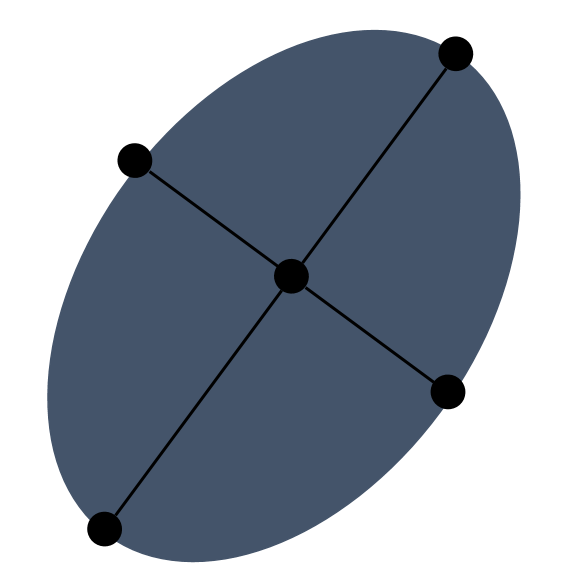
\includegraphics[width=\linewidth]{./ukf1}
	\caption{Initialization of sigma point approximation to the estimate covariance ellipsoid in 2D.}
	\label{fig:ukf1}
	\end{subfigure}
	\hspace{0.04\textwidth}
	\begin{subfigure}[r]{0.35\textwidth}
	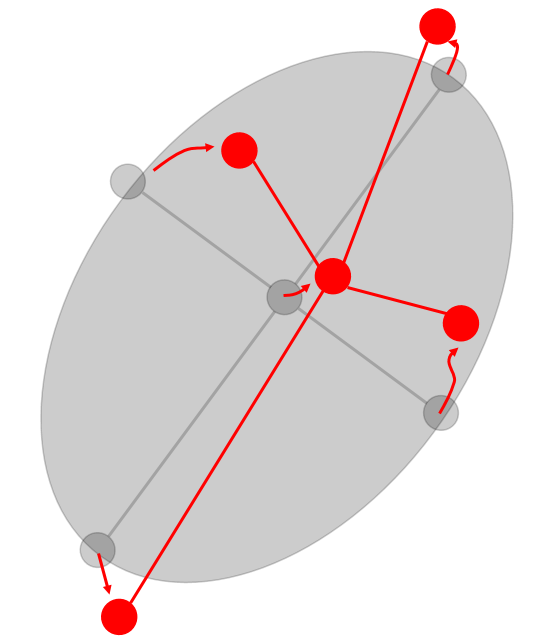
\includegraphics[width=\linewidth]{./ukf2}
	\caption{Propagation of sigma points during the prediction step.}
	\label{fig:ukf2}
	\end{subfigure}
	\\
	\begin{subfigure}[b]{0.35\textwidth}
	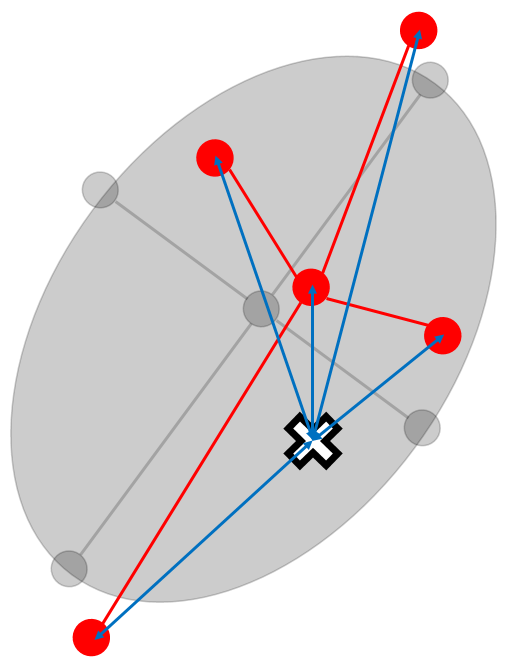
\includegraphics[width=\linewidth]{./ukf3}
	\caption{Computation of the covariance, cross-covariance, and Kalman gain by comparing the prediction sigma points against the measurement.}
	\label{fig:ukf3}
	\end{subfigure}
		\hspace{0.04\textwidth}
	\begin{subfigure}[b]{0.35\textwidth}
	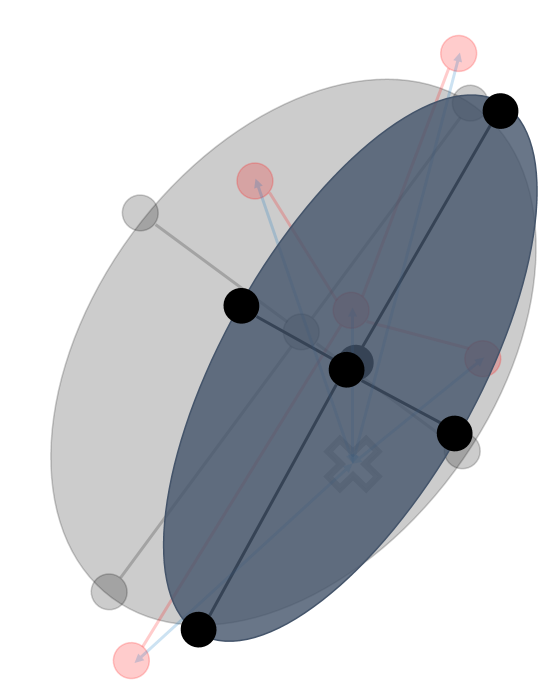
\includegraphics[width=\linewidth]{./ukf4}
	\caption{Re-initialization of sigma points for the next iteration.}
	\label{fig:ukf4}
	\end{subfigure}
	\caption{Graphical summary of the UKF algorithm.}
	\label{fig:ukf_summary}
\end{figure}

A graphical representation of the UKF algorithm is shown in Fig. \ref{fig:ukf_summary} for a 2D random variable.
In the initial step (Fig. \ref{fig:ukf1}), the 2D covariance ellipse is replaced by a particle approximation.
Particles are placed at the mean, and along the positive and negative principal directions.
For the 2D ellipse, this leads to five particles.
Then (Fig. \ref{fig:ukf2}), each of the particles is propagated until the next measurement, using the nonlinear dynamics.
The prediction mean and covariance are determined using a weighted average and weighted variance of the propagated particles.
In Fig. \ref{fig:ukf3}, a measurement is taken (represented by an "X" in the graphic).
The predicted measurement associated with each prediction particle is computed using the nonlinear measurement function.
The measurement is compared against the predicted measurement from the particle values.
The particle predictions are used to approximate a predicted measurement, measurement variance, and cross-covariance between the prediction state and measurement, using weighted means and covariances.
The Kalman gain is computed from these approximations and used to update the prediction mean and variance to a posterior estimate and error variance.
This completes the standard UKF prediction and update cycle.
In Fig. \ref{fig:ukf4}, five new particles are created from the posterior mean and variance, and the filter continues.

A high level-discussion of the UKF has been given; for the full mathematical description, the reader is encouraged to view the appendix.
Now, we turn to a brief comparison of the EKF and UKF, from an application perspective.

Properly implemented, the UKF forms an estimate to a nonlinear process that is at least as good as an EKF estimate.
Due to the higher order approximation implicit in the UKF, it may converge in some cases where an EKF fails.
There is often a tradeoff in terms of computational cost; especially for long state vectors, the EKF algorithm can often exploit matrix sparsity and other linear algebra manipulations to reduce the number of operations required.
The UKF relies upon the nonlinear propagation and measurement expectation of sigma points, and there are fewer opportunities to speed up the computation. 
However, it is true that the UKF and EKF have the same order of computational complexity\cite{wan2000}, making either option much more tractable than methods like particle filters.
The UKF is also somewhat less intuitive for those with a background in analytical estimation.
Finally, although we have not discussed the UKF tuning parameters in this section, they exist and an appropriate choice may not always be obvious.
There don't appear to be well-known automatic or simple heuristic ways to choose those parameters in the literature.

This section has presented the Extended and Unscented Kalman Filters for nonlinear state estimation.
The following section briefly summarizes the overall report.

\section{Summary}

This report has provided background and the underlying algorithm associated with the classical Kalman Filter.
A simple numerical implementation on a linear system has been realized and results shown.
Subsequently, a discussion of two extensions of the Kalman Filter to nonlinear systems have been presented: the Extended Kalman Filter and the Unsceneted Kalman Filter.

%\nocite{kay1993,wan2000,julier1997,woodbury2015,kalman1960,crassidis2011}
\bibliographystyle{plain}
\bibliography{refs}

\appendix
\section{Unscented Kalman Filter: algorithm summary}

The Unscented Kalman Filter algorithm is originally given by Ref. \cite{wan2000}. The notation of the following equations is motivated by Ref. \cite{woodbury2015} as well.
Again, discrete nonlinear dynamics with discrete nonlinear measurements are considered.
Define an augmented state vector as follows:

\begin{equation}
\vecin{x^a}{k} = \begin{bmatrix}
\vecin{x}{k} \\\vecin{w}{k} \\\vecin{v}{k}
\end{bmatrix} \equiv \begin{bmatrix}
\vecin{x^x}{k} \\ \vecin{x^w}{k} \\\vecin{x^v}{k}
\end{bmatrix}
\end{equation}

Note the use of the superscripts $x,w,v$ to denote the entries of the augmented state vector corresponding to the state, process noise, and measurement noise terms, respectively; this notation will be convenient later.
Similarly, define the associated sugmented state covariance matrix:

\begin{equation}
\ten{P^a}(k) \equiv \begin{bmatrix}
\P(k) & 0 & 0\\
0 & \ten{Q}(k) & 0\\
0 & 0 & \ten{R}(k)
\end{bmatrix}
\end{equation}

Denote the length of the augmented state vector as $L$.
Now, define an $L \times (2L+1)$ array of \textit{sigma points}, $\ten{\chi}(k)$.
The $i$th column of $\ten{\chi}(k)$ is defined as follows:

\begin{equation}
\ten{\chi_i}(k)
\begin{cases}
\vecin{x^a}{k} & i = 1\\
\vecin{x^a}{k} + \sqrt{(L+\lambda)}\sqrt{\ten{P^a_i}(k)} & i = 2,\dots,L+1\\
\vecin{x^a}{k} - \sqrt{(L+\lambda)}\sqrt{\ten{P^a_i}(k)} & i = L+2,\dots,2L+1
\end{cases}
\end{equation}

Here, $\sqrt{\ten{P^a_i}(k)}$ is used to denote the $i$th column of the matrix square root of the augmented covariance matrix.
Observe that the sigma point matrix includes perturbed values of the state estimate \textit{as well as of the process and measurement noise vectors.}
Those process and measurement noise elements in the sigma points are passed into the governing dynamics.
Note the presence of $\lambda$, a scalar tuning parameter, that is summarized in the next subsection.
Each column of the sigma point array is a point approximation to the prior, and is passed through the prediction equation as follows to produce a \textit{prediction sigma point array} $\ten{\chi^-}(k+1)$, whose columns are determined as follows:

\begin{equation}
\ten{\chi^-_i}(k+1) = \f(\ten{\chi^x_i}(k),\vecin{u}{k}) + \G(k) \ten{\chi^w_i}(k), i = 1, \dots, 2L+1
\end{equation}

The state and covariance prediction approximations are weighted sums of the propagated sigma points. Denote the mean and covariance weight vectors by $\vec{W^m}$ and $\vec{W^c}$; they are defined separately in the sub-section ``Tuning parameters and weights.''

\begin{equation}
\vecin{\hat{x}^-}{k+1} = \sum_{i=1}^{2L+1} \vec{W^m}(i) \ten{\chi^{x-}_i}(k+1)
\end{equation}
\begin{equation}
\P^-(k+1) = \sum_{i=1}^{2L+1} \vec{W^c}(i) (\ten{\chi^{x-}_i}(k+1)-\vecin{\hat{x}^-}{k+1})(\ten{\chi^{x-}_i}(k+1)-\vecin{\hat{x}^-}{k+1})^T
\end{equation}

For the measurement update step, it is convenient to switch to the index $k$.
Now, the prediction sigma points are each passed through the measurement model, leading to the \textit{measurement sigma point array} $\ten{Y}$:

\begin{equation}
\ten{Y_i}(k) = \h(\ten{\chi^{x-}_i}(k)) + \ten{\chi^{v-}_i}(k)
\end{equation}

The measurement expectation, measurement variance, and prediction-measurement covariance are then approximated by weighted sums:
\begin{align}
\vecin{\hat{y}}{k} \equiv \sum_{i=1}^{2L+1} \vec{W^m}(i) \ten{Y_i}(k) \\
\ten{P_{yy}}(k) \equiv \sum_{i=1}^{2L+1} \vec{W^c}(i) (\ten{Y_i}(k)-\vecin{\hat{y}}{k})(\ten{Y_i}(k)-\vecin{\hat{y}}{k})^T
\\
\ten{P_{xy}}(k) \equiv \sum_{i=1}^{2L+1} \vec{W^c}(i) (\ten{\chi^{x-}_i}(k)-\vecin{\hat{x}^-}{k})(\ten{Y_i}(k)-\vecin{\hat{y}}{k})^T
\end{align}

The Kalman gain is then computed from the variance terms, and the posterior state estimate and variance follow:
\begin{align}
\ten{K}(k) \equiv \ten{P_{xy}}\ten{P_{yy}}^{-1}
\\
\vecin{\hat{x}}{k} = \vecin{\hat{x}^-}{k} + \ten{K}(k)(\vecin{\tilde{y}}{k}-\vecin{\tilde{y}}{k})
\\
\P(k) = \P^-(k) - \ten{K}(k)\ten{P_{yy}}^{-1} \ten{K}^T(k)
\end{align}

The posterior estimate and variance are used to create a new augmented state vector and sigma point matrix, and the process repeats.
The next subsection defines the weights and tuning parameters used in the UKF.

\subsubsection{Tuning parameters and weights}

The mean and covariance weights are selected so that the weighted sums of the prior sigma points is the prior mean and covariance.
The weights are defined as follows:

\begin{equation}
\vec{W^m}(i) = \begin{cases}
\frac{\lambda}{L + \lambda} & i = 1 \\
\frac{1}{2(L+\lambda)} & i = 2, \dots, 2L+1
\end{cases}
\end{equation}
\begin{equation}
\vec{W^c}(i) = \begin{cases}
\frac{\lambda}{L + \lambda}+(1-\alpha^2+\beta) & i = 1 \\
\frac{1}{2(L+\lambda)} & i = 2, \dots, 2L+1
\end{cases}
\end{equation}

$\beta$ is used to incorporate prior knowledge of the ``true'' distribution; $\beta = 2$ is optimal for Gaussian priors.

$\lambda$ is defined as follows.
$\alpha$ determines the spread of the sigma points about the mean and is generally set to a small value, say $10^{-3}$.
$\kappa$ is a ``secondary scaling parameter,'' and is commonly set to zero [2].

\begin{equation}
\lambda = \alpha^2(L+\kappa)-L
\end{equation}

\end{document}
